
\subsection{Multi-Layer Perceptron}

Multi-Layer Perceptron (MLP) là một loại mạng nơ-ron nhân tạo, là một phần của học sâu (deep learning). MLP bao gồm ít nhất ba lớp: một lớp đầu vào, một hoặc nhiều lớp ẩn, và một lớp đầu ra. Mỗi lớp chứa nhiều nơ-ron (neurons), và mỗi nơ-ron trong một lớp kết nối với tất cả các nơ-ron trong lớp kế tiếp.

MLP có thể được sử dụng cho nhiều nhiệm vụ khác nhau như phân loại, hồi quy và dự báo chuỗi thời gian. Mỗi nơ-ron trong MLP sử dụng một hàm kích hoạt phi tuyến tính để tạo ra đầu ra của nó, giúp mạng có khả năng học các mối quan hệ phi tuyến giữa đầu vào và đầu ra.
\begin{figure}[h]
    \centering
    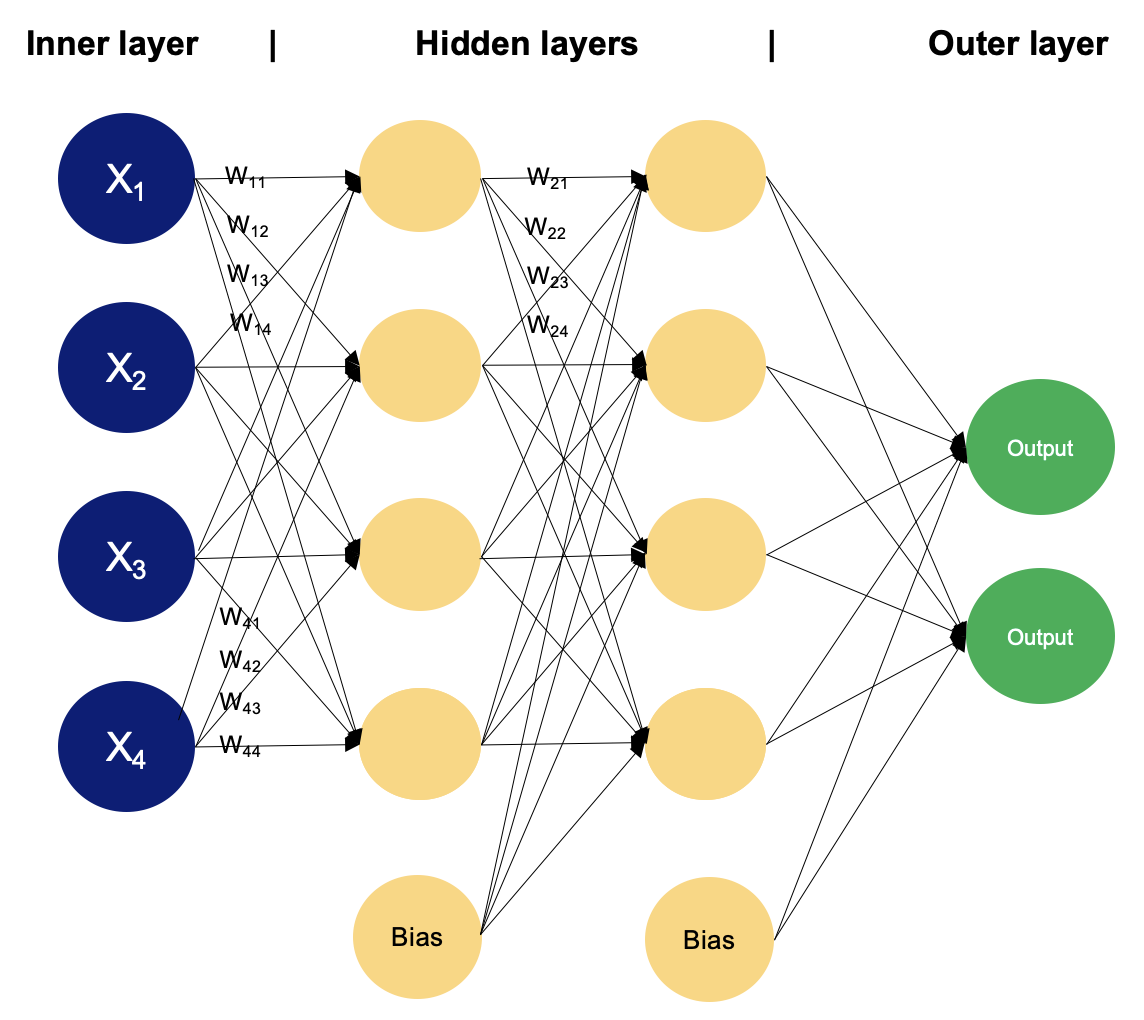
\includegraphics[width=0.3\textwidth, height=0.3\textwidth]{img/MLP.png}
    \caption{Ví dụ về MLP có hai lớp ẩn}
    \label{fig:your_figure_label}
\end{figure}

\subsubsection{Mô tả thuật toán}
Mạng Perceptron Đa Lớp là một loại mạng nơ-ron nhân tạo (Artificial Neural Network - ANN) bao gồm nhiều lớp perceptron được sắp xếp theo cấu trúc phân tầng. Cấu trúc của MLP thường bao gồm ba loại lớp chính:

\begin{itemize}
    \item \textbf{Lớp đầu vào (Input Layer)}: Đây là lớp nhận các giá trị đầu vào và truyền chúng vào các lớp tiếp theo. Số lượng nơ-ron trong lớp này tương ứng với số lượng tính năng của dữ liệu đầu vào.
    \item \textbf{Lớp ẩn (Hidden Layer)}: MLP có thể có một hoặc nhiều lớp ẩn. Các lớp này chịu trách nhiệm học các đặc trưng phức tạp của dữ liệu. Mỗi nơ-ron trong lớp ẩn nhận đầu vào từ tất cả các nơ-ron của lớp trước đó và áp dụng một hàm kích hoạt (activation function) để xác định giá trị đầu ra.
    \item \textbf{Lớp đầu ra (Output Layer)}: Lớp này cung cấp kết quả cuối cùng của mạng. Số lượng nơ-ron trong lớp đầu ra phụ thuộc vào số lượng lớp mục tiêu (target classes) trong bài toán phân loại hoặc số lượng biến mục tiêu trong bài toán hồi quy.
\end{itemize}

Công thức cơ bản cho một nơ-ron trong lớp ẩn hoặc lớp đầu ra là:
\[
y = f\left( \sum_{i=1}^{n} w_i \cdot x_i + b \right)
\]

Trong đó:
\begin{itemize}
    \item \( y \) là đầu ra của nơ-ron.
    \item \( f \) là hàm kích hoạt (chẳng hạn như hàm sigmoid, tanh, hoặc ReLU).
    \item \( x_i \) là các đầu vào.
    \item \( w_i \) là các trọng số liên kết với các đầu vào.
    \item \( b \) là hệ số điều chỉnh (bias).
\end{itemize}

\subsubsection{Thuật Toán Gradient Descent}

Gradient descent là một phương pháp tối ưu hóa phổ biến được sử dụng để tìm cực tiểu của hàm mất mát (loss function). Trong ngữ cảnh của MLP, hàm mất mát đo lường sự khác biệt giữa dự đoán của mạng và giá trị thực tế.
Công thức cập nhật trọng số trong gradient descent như sau:
\[
\theta_{i} := \theta_{i} - \eta \frac{\partial J(\theta)}{\partial \theta_{i}}
\]
trong đó, \(\theta_{i}\) là trọng số cần cập nhật, \(\eta\) là tốc độ học (learning rate), và \(J(\theta)\) là hàm mất mát.

\subsubsection{Thuật toán Backpropagation}

Backpropagation là một phương pháp hiệu quả để tính gradient của hàm mất mát đối với các trọng số của MLP. Quá trình backpropagation bao gồm hai bước chính: lan truyền tiến (forward propagation) và lan truyền ngược (backward propagation).

Trong bước lan truyền tiến, chúng ta tính toán đầu ra của mạng cho một đầu vào cụ thể. Trong bước lan truyền ngược, chúng ta tính toán gradient của hàm mất mát đối với từng trọng số bằng cách áp dụng quy tắc dây chuyền (chain rule).

\subsubsection{Feedforward}

Feedforward là quá trình tính toán đầu ra của mạng từ đầu vào bằng cách đi qua các lớp nơ-ron. Quá trình này bao gồm việc tính toán đầu ra của mỗi nơ-ron trong lớp ẩn và lớp đầu ra.

Giả sử \(a^{(l)}\) là đầu ra của lớp \(l\), quá trình feedforward được mô tả như sau:
\[
z^{(l+1)} = W^{(l)}a^{(l)} + b^{(l)}
\]
\[
a^{(l+1)} = \sigma(z^{(l+1)})
\]
trong đó, \(W^{(l)}\) và \(b^{(l)}\) lần lượt là trọng số và bias của lớp \(l\), \(z^{(l+1)}\) là tổng trọng số, và \(\sigma\) là hàm kích hoạt.